\subsection{Beam energy}
We estimated a beam momentum using simple MC simulation.
Figure \ref{K11Br_Beam_line} shows MC simulation's geometry.
We generate 800MeV/$c$ pencil beam and shoot the beam downstream.
Figure \ref{k_pi_momentum} shows Kaon and Pion momentum distribution
using this MC simulation at BDC.
Kaon beam momentum is estimated by the momentum distribution of MC simulation.
%Actually, kaon momentum distribution peak is adjusted so that kaon decay point of MC simulation is consistent with data.
%Section \ref{kaon_energy_section} explains this point.
%And proton momentum is estimated in other way, using TREK detector TOF information.
%Section \ref{proton_energy_section} shows proton momentum distribution.

\begin{figure}[!htb]
  \centering
  \centering
  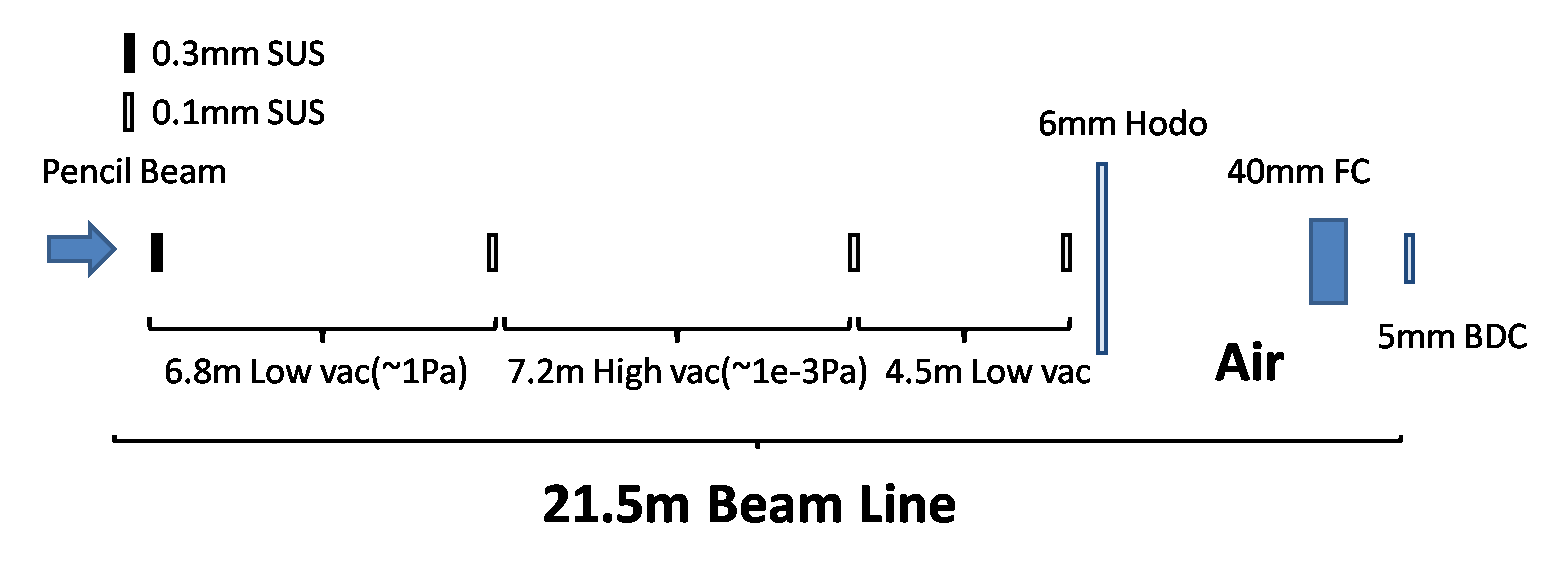
\includegraphics[width=10cm,clip]{./fig/K11Br_beamline_sim.eps}
  \caption{K1.1 Br beam line}
  \label{K11Br_Beam_line}
\end{figure}


\begin{figure}[!htb]
  \centering
  \centering
  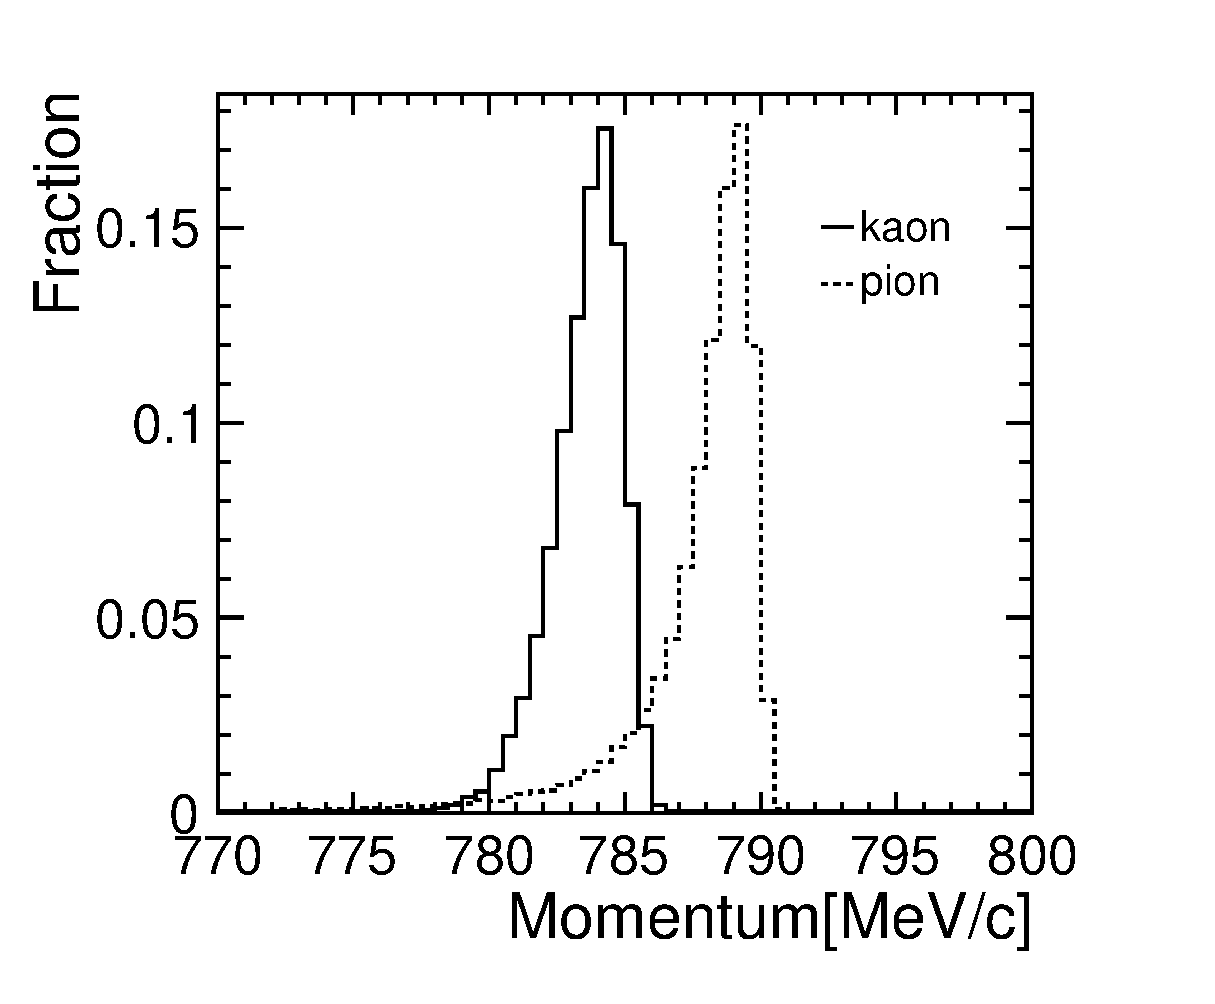
\includegraphics[width=10cm,clip]{./fig/Kaon_pion_momentum_nogrid.eps}
  \caption{Kaon and Pion momentum distribution at BDC}
  \label{k_pi_momentum}
\end{figure}


\subsubsection{Kaon energy
  \label{KaonEnergy}
}
Kaon beam momentum is estimated by the momentum distribution of MC simulation.
We change Kaon beam momentum in a range of 700 - 800 MeV/$c$ and search the momentum that decay point distribution of MC simulation is consistent with data one.

\subsubsection{Proton energy}
Proton momentum shown in Figure \ref{fig:Proton_momentum} is used as proton beam momentum of MC simulation.

\subsubsection{Energy deposition in degrader}
It is too high energy that Kaon beam stops in the fiducial volume of 250LAr TPC.
In order to degrade the beam momentum, some lead glass blocks and a lead brick were inserted in front of 250LAr TPC as degrader.
%We estimate energy deposition in degrader by using MC simulation.
Figure \ref{energy_deposition} shows energy deposition distribution in degrader.


\begin{figure}[!htb]
  \centering
  \centering
  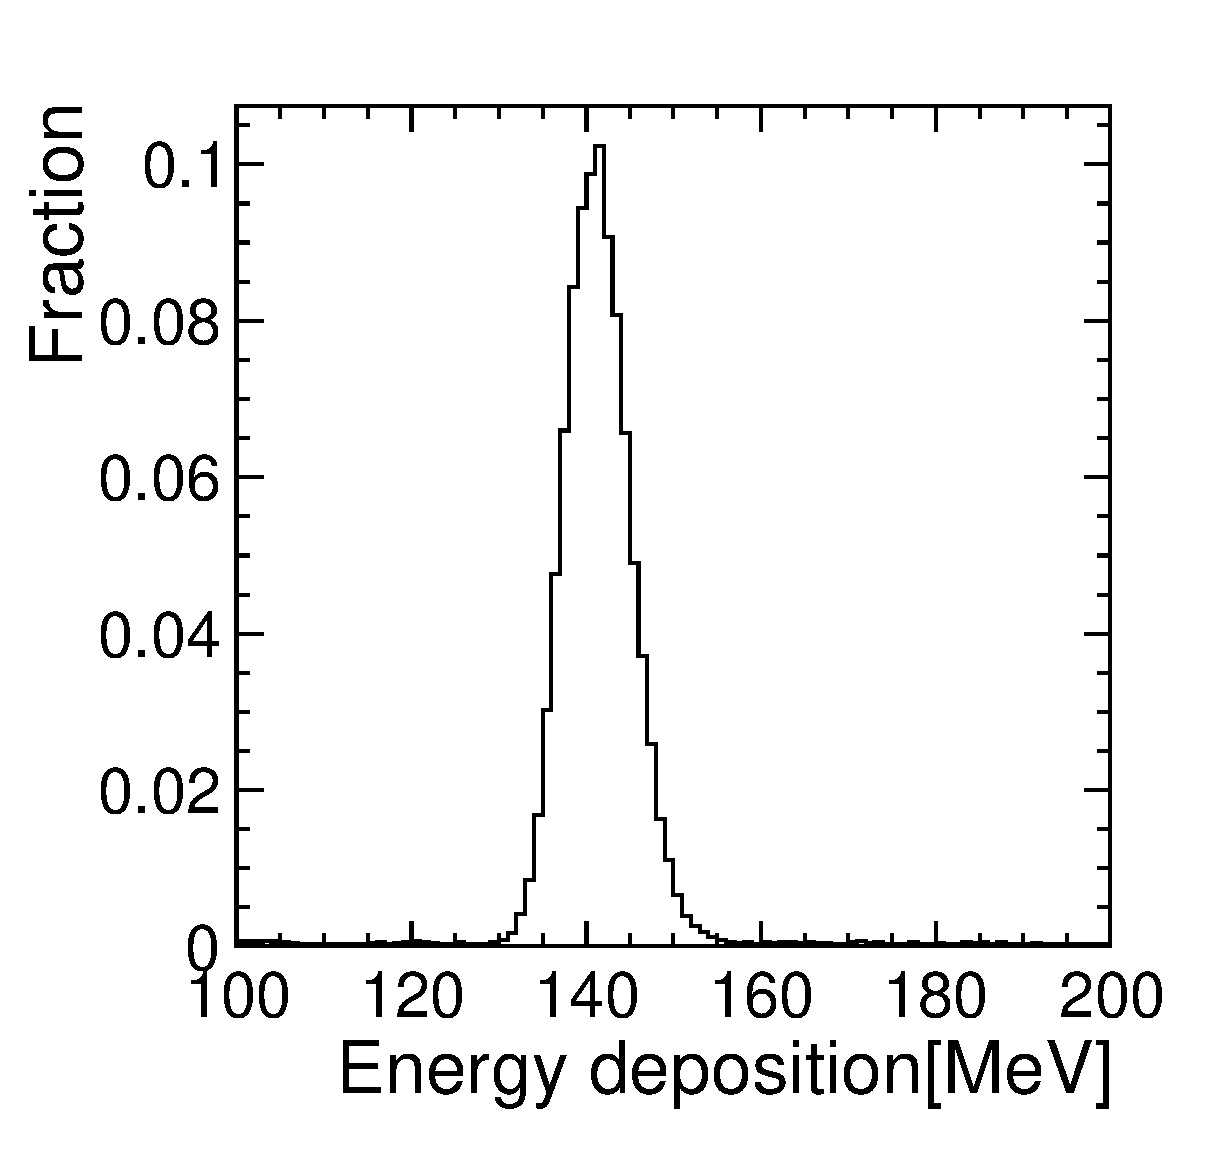
\includegraphics[width=10cm,clip]{./fig/energy_deposition.eps}
  \caption{Energy deposition in degrader}
  \label{energy_deposition}
\end{figure}




